Die Oberfläche einer Wasserkugel vom Radius 1 geht beim $x=0$ durch die 
optische Achse.
An ihr wird ein achsparalleler Lichtstrahl gebrochen.
Wasser hat Brechungsindex $n=\frac{4}{3}$.
\begin{teilaufgaben}
\item
Wie lautet die Brechungsmatrix
\item
Man betrachte einen achsparallelen Strahl durch den Punkt $(0,1)$
Bei welcher $x$-Koordinate schneidet der gebrochene Strahl die Achse?
\end{teilaufgaben}


\begin{loesung}
\begin{center}
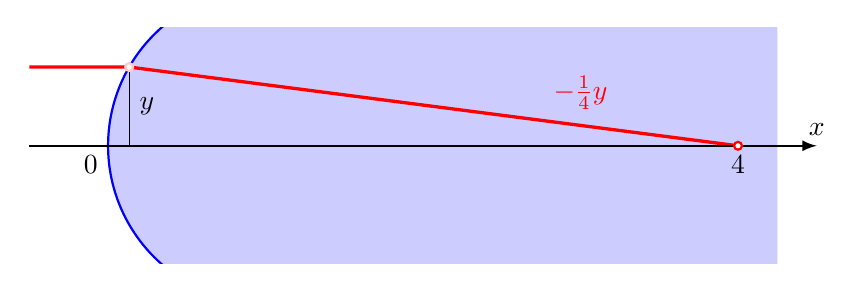
\begin{tikzpicture}[>=latex,thick]
\def\y{1}
\def\R{2}
\begin{scope}
\clip ({-\R-1},-1.5) rectangle ({3*\R+0.5},1.5);
\fill[color=blue!20] (0,0) circle[radius=\R];
\draw[color=blue] (0,0) circle[radius=\R];
\fill[color=blue!20] (0,-3) rectangle (10,3);
\end{scope}
\draw[line width=0.3pt] ({-sqrt(\R*\R-\y*\y)},0) -- ++(0,\y);
\node at ({-sqrt(\R*\R-\y*\y)},{0.5*\y}) [right] {$y$};
\draw[line width=1.2pt,color=red] ({-\R-1},\y)
	-- ({-sqrt(\R*\R-\y*\y)},\y)
	-- ({3*\R},0);
\fill[color=white] ({-sqrt(\R*\R-\y*\y)},\y) circle[radius=0.05];
\draw[color=red!20] ({-sqrt(\R*\R-\y*\y)},\y) circle[radius=0.05];
\draw[->] ({-\R-1},0) -- ({3*\R+1},0) coordinate[label={$x$}];
\fill[color=white] ({3*\R},0) circle[radius=0.05];
\draw[color=red] ({3*\R},0) circle[radius=0.05];
\node[color=red] at ({2*\R},{0.333*\y}) [above] {$-\frac14y$};
\node at ({-\R},0) [below left] {$0$};
\node at ({3*\R},0) [below] {$4$};
\end{tikzpicture}
\end{center}
\begin{teilaufgaben}
\item
Da der Brechungsindex $n_1$ von Luft vernachlässigt werden kann, muss nur der
Brechungsindex $n_2=n=\frac43$ von Wasser berücksichtigt werden.
Die Brechungsmatrix  ist dann
\begin{align*}
B(n_1,n_2,R)
&=
\begin{pmatrix}
1&0\\
\frac{1}{R}\left(\frac{n_1}{n_2}-1\right) & \frac{n_1}{n_2}
\end{pmatrix}
\\
B(1,{\textstyle\frac43},1)
&=
\begin{pmatrix}
1&0\\
\frac{3}{4}-1 & \frac{3}{4}
\end{pmatrix}
=
\begin{pmatrix}
1&0\\
-\frac{1}{4} & \frac{3}{4}
\end{pmatrix}
\end{align*}
\item
Der Ausgangsstrahl wird durch den Vektor
\[
\begin{pmatrix}y\\0\end{pmatrix}
\]
beschrieben.
Der gebrochene Strahl ist daher
\[
B(1,{\textstyle\frac43},1)
\begin{pmatrix}
1\\0
\end{pmatrix}
=
\begin{pmatrix}
1&0\\
-\frac{1}{4} & \frac{3}{4}
\end{pmatrix}
\begin{pmatrix}
y\\0
\end{pmatrix}
=
\begin{pmatrix}
y\\
-\frac14y
\end{pmatrix}.
\]
Der gebrochene Strahl hat daher die Steigung $-\frac14y$ und schneidet die
$x$-Achse beim Punkt $x=4$.
\qedhere
\end{teilaufgaben}
\end{loesung}
